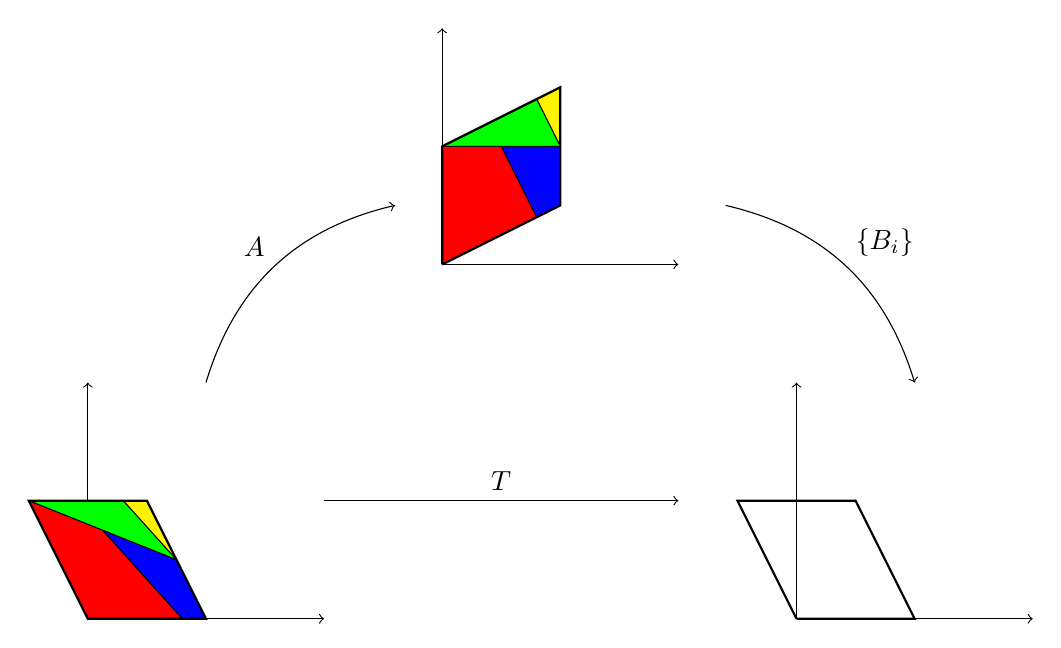
\begin{tikzpicture}[scale=1.5]
    % Parallelogram 1

    % initial axis
    \draw[<->, thin] (2,0) -- (0,0) -- (0,2);

    \coordinate (a1) at (0,0);
    \coordinate (b1) at (1,0);
    \coordinate (c1) at (0.5,1);
    \coordinate (d1) at (-0.5,1);

    \coordinate (a1b1) at (4/5, 0);
    \coordinate (x1) at (1/8, 3/4);
    \coordinate (b1c1) at (3/4, 1/2);
    \coordinate (c1d1) at (3/10, 1);

    \fill[red] (a1) -- (a1b1) -- (x1) -- (d1) -- cycle;
    \fill[blue] (a1b1) -- (b1) -- (b1c1) -- (x1) -- cycle;
    \fill[green] (b1c1) -- (c1d1) -- (d1) -- cycle;
    \fill[yellow] (b1c1) -- (c1) -- (c1d1) -- cycle;

    % cuts
    \draw (a1b1) -- (x1) (b1c1) -- (c1d1) (b1c1) -- (d1);

    % contour
    \draw[thick] (a1) -- (b1) -- (c1) -- (d1) -- cycle;

    % Environment for parallelogram 2
    \begin{scope}[xshift=3cm,yshift=3cm]
        \draw[<->, thin] (2,0) -- (0,0) -- (0,2); % assi

        \coordinate (a2) at (0,0);
        \coordinate (b2) at (1,0.5);
        \coordinate (c2) at (1,1.5);
        \coordinate (d2) at (0,1);

        \coordinate (a2b2) at (4/5, 2/5);
        \coordinate (x2) at (1/2, 1);
        \coordinate (b2c2) at (1, 1);
        \coordinate (c2d2) at (4/5, 7/5);

        \fill[red] (a2) -- (a2b2) -- (x2) -- (d2) -- cycle;
        \fill[blue] (a2b2) -- (b2) -- (b2c2) -- (x2) -- cycle;
        \fill[green] (b2c2) -- (c2d2) -- (d2) -- cycle;
        \fill[yellow] (b2c2) -- (c2) -- (c2d2) -- cycle;

        % cuts
        \draw (a2b2) -- (x2) (b2c2) -- (c2d2) (b2c2) -- (d2);

        % contour
        \draw[thick] (a2) -- (b2) -- (c2) -- (d2) -- (a2);
    \end{scope}

    % Environment for parallelogram 3
    \begin{scope}[xshift=6cm]
        \draw[<->, thin] (2,0) -- (0,0) -- (0,2); % assi

        \coordinate (a3) at (0,0);
        \coordinate (b3) at (1,0);
        \coordinate (c3) at (0.5,1);
        \coordinate (d3) at (-0.5,1);

        \draw[thick] (a3) -- (b3) -- (c3) -- (d3) -- (a3);
    \end{scope}

    % arrow 1 -> 2
    \draw[->] (1,2) to [bend left] node [midway, above left] { $ A $ } (2.6, 3.5);

    % arrow 2 -> 3
    \draw[->] (5.4,3.5) to [bend left] node [midway, above right] { $ \{B_i\} $ } (7,2);

    % arrow 3 -> 1
    \draw[<-] (5,1) to [] node [midway, above] { $ T $ } (2,1);
\end{tikzpicture}
